\xiti
\begin{xiaotis}

\xiaoti{用较厚的纸按照图的样子画好剪下,再把它折起来粘好,做成棱柱的模型(选做其中一个)。}

\begin{figure}[H]%[htbp]
    \centering
    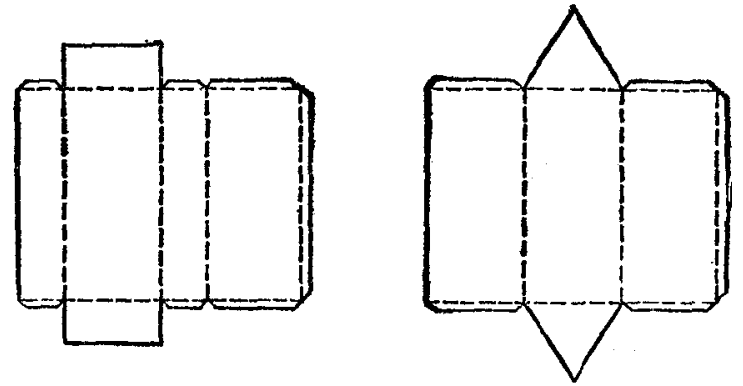
\includegraphics[width=10cm]{../pic/ltjh-ch2-xiti7-01.png}
    \caption*{(第 1 题)}
\end{figure}

\xiaoti{底面是菱形的直棱柱,对角线 $B'D$ 和 $A'C$ 的长分别是 9 cm 和 15 cm,侧棱 $AA'$ 的长是 $5\;\limi$。 求它的底面边长。}

\begin{figure}[htbp]
    \centering
    \begin{minipage}[b]{5cm}
        \centering
        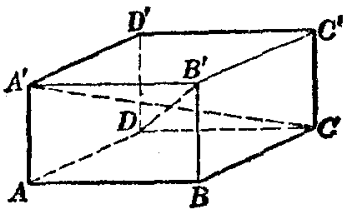
\includegraphics[width=5cm]{../pic/ltjh-ch2-xiti7-02.png}
        \caption*{(第 2 题)}
    \end{minipage}
    \qquad
    \begin{minipage}[b]{4cm}
        \centering
        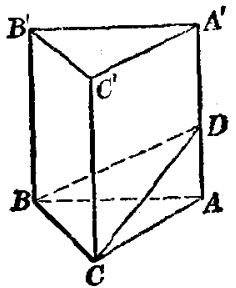
\includegraphics[width=3.5cm]{../pic/ltjh-ch2-xiti7-03.png}
        \caption*{(第 3 题)}
    \end{minipage}
    \qquad
    \begin{minipage}[b]{4cm}
        \centering
        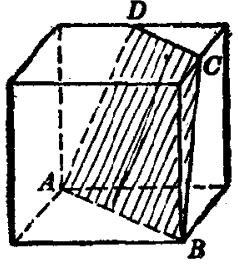
\includegraphics[width=4cm]{../pic/ltjh-ch2-xiti7-13.png}
        \caption*{(第 13 题)}
    \end{minipage}
\end{figure}

\xiaoti{如图,正三棱往的底面边长是 4 cm,过 $BC$ 的一个平面与底面成 $30^\circ$ 的二面角,
    交侧棱 $AA'$ 于 $D$。求 $AD$的长和截面 $\triangle BCD$ 的面积。
}

\xiaoti{求证:}
\begin{xiaoxiaotis}

    \xxt{平行六面体的各对角线交于一点,并且在这一点互相平分;}

    \xxt{对角线相等的平行六面体是长方体。}

\end{xiaoxiaotis}


\xiaoti{有一个长方体,它的三个面的对角线长分别是 $a$、$b$、$c$。求它的对角线长。}

\xiaoti{长方体的一条对角线与各个面所成的角分别是 $\alpha$、$\beta$、$\gamma$。
    求证: $\cos^2\alpha + \cos^2\beta + \cos^2\gamma = 2$。
}

\xiaoti{已知一个正五棱柱的高是 4 cm,底面外接圆的半径是 2.5 cm,画它的直观图(不写画法)。}

\xiaoti{求证:直三棱柱的两个侧面的面积的和,大于第三个侧面的面积。}

\xiaoti{直平行六面体的底面是菱形,过不相邻的两对侧棱的截面的面积是 $Q_1$ 和 $Q_2$,求它的侧面积。}

\xiaoti{一个长方体的三条棱长的比是 $1:2:3$,全面积是 $88\;\pflm$。求这三条棱的长。}

\xiaoti{除锈滚筒是正六棱柱形(两端是封闭的),简长 1.6 m,底面外接圆半径是 0.46 m,
    制造这个滚筒需要多少平方米铁板?(精确到 $0.1\;\pfm$)
}

\xiaoti{在正三棱柱的一条侧棱上,取距离等于 $a$ 的两点,过这两点作两个与所有的侧棱都相交的互相平行的截面,
    如果正三棱柱的底面边长为 $b$,求棱柱的侧面夹在这两个平行截面间的部分的面积。
}

\xiaoti{如图,正方体的棱长为 $a$,$C$、$D$ 分别是两条棱的中点。
    (1)试证 $A$、$B$、$C$、$D$ 在同一平面内;
    (2)求截面 $ABCD$ 的面积。
}

\end{xiaotis}


